\documentclass{beamer}
\usefonttheme{serif}
\usetheme{boadilla}

\usepackage{amsthm, amsfonts, amsmath, amssymb} % Pacote para a definicao dos ambientes matematicos
\usepackage[brazilian]{babel}
\usepackage[utf8]{inputenc}
\usepackage[mathscr]{eucal}
\usepackage{tikz}
\usepackage{subcaption}
\usepackage{graphicx}
\usepackage{hyperref}
\usetikzlibrary{quotes, angles, intersections}
\newcommand{\R}{\mathbb{R}}
\newcommand{\D}{\mathscr{D}}
\newcommand{\Pp}{\mathscr{P}}
\newcommand{\bigO}{\mathscr{O}}
\newcommand{\Cc}{\mathscr{C}}
\newcommand{\E}{\mathscr{E}}
\newcommand{\F}{\mathscr{F}}
\newcommand{\Ww}{\mathscr{W}}
\newcommand{\Rr}{\mathscr{R}}
\newcommand{\norm}[2][2]{\left\lVert#2\right\rVert_{#1}}
\newcommand{\sigla}[2]{#2 (#1)}
\newcommand{\citeonline}[1]{\cite{#1}}

\newtheorem{thm}{Theorem}
\newtheorem{prp}{Proposition}
\newtheorem{lem}{Lemma}
\theoremstyle{definition}
%\newtheorem{definition}{Definition}[section]

\author{Danilo Tedeschi}
\title{New Exact Algorithms for Planar Maximum Covering Location by Ellipses Problems}
\institute{Universidade de São Paulo}
\date{25 de Outubro de 2019}


\begin{document}
	
	\begin{frame}[t,plain]
		\titlepage
		
		\footnotesize This research has been funded by Cordenação de Aperfeiçoamento de Pessoal de Nível Superior (CAPES).
	\end{frame}

	\begin{frame}{Introduction}{Related problems}

		\sigla{MCLP}{The Maximum Covering Location Problem} 
		\begin{itemize}
			\item Introduced in \cite{church:1974},
			\item Maximize the coverage demand vertices on a graph,
			\item Choose the location (vertex) of a fixed number of facilities,
			\item A demand vertex is considered covered if a facility is located within its coverage radius.
		\end{itemize}
	\end{frame}

	\begin{frame}{Introduction}{Related problems}
	
	\sigla{PMCLP}{The Planar Maximum Covering Location Problem} 
	\begin{itemize}
		\item Introduced in \cite{church:1984},
		\item Maximize the coverage demand vertices in $\R^2$,
		\item Choose the location (could be anywhere in $\R^2$) of a fixed number of facilities,
		\item A demand vertex is considered covered if a facility is located within its coverage radius,
		\item Several distance functions were studied. We are particularly interested in the Euclidean PMCLP.
	\end{itemize}
	\end{frame}

\begin{frame}{Introduction}
	
	We propose algorithms for two versions of PMCLP.
	
\end{frame}

\begin{frame}{Introduction}{MCE}
	Planar Maximum Covering Location by Ellipses Problem (MCE):
	\begin{itemize}
		\item Introduced in \cite{canbolat}, 
		\item Mixed Non-linear optimization and a heuristic method in \cite{canbolat},
		\item Exact method, solving convex sub-problems in \cite{andreta}.
	\end{itemize}

	\begin{block}{Our algorithm}		
		Based on the approach used for the Euclidean PMCLP in \cite{church:1984}.
		Transform MCE into a combinatorial optimization problem.
	\end{block}
\end{frame}

\begin{frame}{Introduction}{MCER}
	Planar Maximum Covering Location by Ellipses with Rotation Problem (MCER):
	\begin{itemize}
		\item Introduced in \cite{andreta}, 
		\item Exact method, solving many optimization sub-problems in \cite{canbolat},
		\item Heuristic method in \cite{andreta}.
		\item Much more challenging than MCE.
	\end{itemize}
	
	\begin{block}{Our algorithm}		
		Transforms MCER into a combinatorial optimization problem.
	\end{block}
\end{frame}

\begin{frame}{Introduction}{Ellipse}
	The shape of an ellipse is given by its major-axis and minor-axis, $(a, b) \in \mathbb{R}^2_{>0}$, $a > b$.
	
	\begin{figure}[H]
		\centering
		
		%\caption{The ellipse as a parametric curve.}
		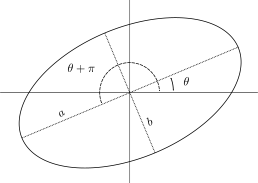
\includegraphics[scale=.3]{../tex/figures/rotated_ellipse.pdf}
		\label{fig:ellipse_params}
		\caption{An ellipse with shape parameters $a$ and $b$.}
	\end{figure}
	
\end{frame}

\begin{frame}{Introduction}{Ellipse}
	An ellipse can be defined using a norm function $||\cdot||_{a,b,\theta}$ given by
	\begin{equation*}
		||x||_{a,b, \theta}=\left|\left|
		\left(\begin{array}{rr}
		\cos{\theta} & \sin{\theta}\\
		\sin{\theta} & -\cos{\theta}
		\end{array}
		\right)
		\left(\begin{array}{cc}
		1/a & 0\\
		0 & 1/b
		\end{array}\right) x \right|\right|_2.
	\end{equation*}
\end{frame}

\begin{frame}{Problem definition}
	%\begin{block}{Definition}
	An instance of both MCE and MCER is given by
	\begin{itemize}
		\item A demand set $\Pp:=\{p_1, \dots, p_n\}$, $p_j \in \R^2$;
		\item Each point has a weight $\Ww := \{w_1, \dots, w_n\}$, $w_j \in \R_{\ge0}$;
		\item A list of shape parameters $\Rr := \{(a_1, b_1); \dots; (a_m, b_m)\}$, $(a_j, b_j) \in \R^2_{>0}$, with $a_j > b_j$.
	\end{itemize}
\end{frame}

\begin{frame}{Problem definition}
	\begin{figure}
		\begin{subfigure}{.4\textwidth}
			\centering
			\includegraphics[scale=.55]{../article/figures/MCE_TA04}
			\caption{}
			\label{fig:MCE_TA04}
		\end{subfigure}
		\begin{subfigure}{.4\textwidth}
			\centering
			\includegraphics[scale=.55]{../article/figures/MCER_TA04}
			\caption{}
			\label{fig:MCER_TA04}
		\end{subfigure}
		\caption{Solutions for the same instance of (a) MCE, and (b) MCER.}
		\label{fig:TA04}
	\end{figure}
\end{frame}

\begin{frame}{Problem definition}{More notation}
	
	\begin{block}{Weight function}
	Let $w\colon 2^\Pp \to \R$ be a function defined as
	
	\begin{equation*}
	w(A) = \sum_{j \colon p_j \in A} w_j.
	\end{equation*}
	
%	which takes a subset of $\Pp$ and returns the sum of the weights of the points in that subset.
	\end{block}

\begin{block}{MCE's solution}
	$Q:=(q_1, \dots, q_m) \in \R^{2m}$.
\end{block}

\begin{block}{MCER's solution}
	%$Q:=(q_1, \dots, q_m)$.\\
	$Q:=((q_1, \theta_1); \dots; (q_m, \theta_m)) \in (\R^2\times [0, \pi))^m$.
\end{block}
	
	%(Only used to make the text more clear)
\end{frame}

\begin{frame}{Problem definition}{MCE}
	Let $E_j \colon \R^2 \to \R^2$ be the coverage region of the $j$-th ellipse defined as
	\begin{equation*}
	E_j(q) = \{x \in \R^2\colon ||x-q||_{a,b,0} \le 1\}.
	\end{equation*}
	Then, MCE is defined as the optimization problem:
	\begin{equation*}
	\max_{Q}  w\left(\bigcup_{j=1}^m\Pp \cap E_j(q_j)\right).
	\end{equation*}
\end{frame}

\begin{frame}{Problem definition}{MCER}
	Let $E_j \colon \R^2\times[0, \pi) \to \R^2$ be the coverage region of the $j$-th ellipse defined as
	\begin{equation*}
	E_j(q,\theta) = \{x \in \R^2\colon ||x-q||_{a,b,\theta} \le 1\}.
	\end{equation*}
	Then, MCER is defined as the optimization problem:
	\begin{equation*}
	\max_{Q}  w\left(\bigcup_{j=1}^m\Pp \cap E_j(q_j,\theta_j)\right).
	\end{equation*}
	
	\begin{block}{Remark}
		For the one-facility MCE and MCER, we omit the index referring to the ellipse.
	\end{block}
\end{frame}

\begin{frame}{MCE}
	$\{p_1, p_2, p_3\} \subset E(q)$
	\begin{figure}
		\centering
		\includegraphics[scale=.55]{figures/mce-mwc0}
		\caption{A solution for the one-facility MCE.}
	\end{figure}
\end{frame}

\begin{frame}{MCE}
	$\{p_1, p_2, p_3\} \subset E(q) \implies q \in E(p_1) \cap E(p_2) \cap E(p_3)$.
	\begin{figure}
		\centering
		\includegraphics[scale=.55]{figures/mce-mwc}
		\caption{A solution for the one-facility MCE.}
	\end{figure}
\end{frame}

\begin{frame}{MCE}
	In general we have
	\begin{equation*}
	A = \Pp \cap E(q) \implies 	q \in \cap_{p \in A} E(p),
	\end{equation*}
and
	\begin{equation*}
	q' \in \cap_{p \in A} E(p) \implies	A \subset E(q').
	\end{equation*}
	
	\begin{block}{Intersection region of ellipses}
		By \cite{bi}, we have that if $|A|>1$, there is at least one intersection between two ellipses in the border of $\cap_{p\in A} E(p)$.
	\end{block}
\end{frame}

\begin{frame}{MCE}
	$\{q_1, q_2, q_3\} \subset \bigcup_{1 \le i < j \le 3} \partial E(p_i) \cap \partial E(p_j)$.
	\begin{figure}
		\centering
		\includegraphics[scale=.55]{figures/mce-mwc1}
		\caption{A solution for the one-facility MCE.}
	\end{figure}
\end{frame}

\begin{frame}{MCE}
	In general, we have
	\begin{equation*}
	|\partial E(u) \cap \partial E(v)| \le 2, 
	\end{equation*}
	and that $\partial E(u) \cap \partial E(v)$ can be determined analytically.
\end{frame}

\begin{frame}{MCE}{Candidate List Set}
	
	Based on \cite{church:1984}, we define a Candidate List Set (CLS) for each facility as follows.
	
	\begin{definition}\label{def:cls_mce}
		Given an instance of MCE, for all $k \in \{1, \dots, m\}$, we define the CLS for the $k$-th ellipse as
		\begin{equation*}
		S_k = \Pp \cup \left(\bigcup_{1 \le i < j \le n} \partial E_k(p_i) \cap \partial E_k(p_j) \right).
		\end{equation*}
	\end{definition}
\end{frame}

\begin{frame}{MCE}{Main result}
	\begin{thm}\label{thm:mce}
		Given an instance of MCE, and $S_1, \dots, S_m$ as defined previously, then the set $$\Omega = \{(q_1, \dots, q_m) \colon \textnormal{ for all }q_k \in S_k \}$$ contains an optimal solution of MCE and $|\Omega| \le n^{2m}$. 
	\end{thm}

\begin{itemize}
	\item Notice that $|S_k| \le n(n+1)/2 \le n^2$.
	\item An algorithm with $\bigO(mn^{2m+1})$ runtime complexity can be implemented.
\end{itemize}

\end{frame}


%%% E3P

\begin{frame}{Determining Every Center and Angle of Rotation of An Ellipse Given Its Shape and Three Points that It Must Contain}
	Given
	\begin{itemize}
		\item The coverage region function of an ellipse $E \colon \R^2 \times [0, \pi) \to \R^2$.
		\item Three points $u, v, w \in \R^2$.
	\end{itemize}
Let us call E3P the problem whose solution is given by $(q, \theta) \in \R^2 \times [0, \pi)$, such that

$$\{u, v, w\} \subset \partial E(q, \theta).$$

We want to compute every solution of E3P.

We did not find any work on E3P in the literature.
\end{frame}

\begin{frame}{E3P}
	\begin{figure}
		\centering
		\includegraphics[scale=.4]{../tex/figures/e3p_4sols}
		\caption{Example of every solution for an instance of E3P.}
	\end{figure}
\end{frame}

\begin{frame}{E3P}{Transforming the problem}
	Let us define a function $\varphi \colon \R^2 \times [0, \pi) \to \R^2$ that transforms the problem as follows.
	\begin{figure}
		\centering
		\includegraphics[scale=.7]{../article/figures/circumscribed-circle}
		\caption{Transforming a solution of E3P into a solution of the circumcircle problem.}
	\end{figure}
\end{frame}

\begin{frame}{E3P}{Transforming the problem}
	If $u$ is at the origin, this function can be described as
	\begin{equation*}%\label{eq:trpnts}
	\varphi(p, \theta)=\left[\begin{array}{cc}
	\frac{b}{a}&0\\
	0&1
	\end{array}\right]
	\left[\begin{array}{cc}
	\cos{\theta}&\sin{\theta}\\
	-\sin{\theta}&\cos{\theta}
	\end{array}\right]\left[\begin{array}{c}
	p_x\\
	p_y
	\end{array}\right].
	\end{equation*}
	
	\begin{itemize}
		\item For a fixed angle, $\varphi$ is bijective, we refer to $\varphi^{-1}$ as its inverse.
		\item Let us denote by $\Lambda(\theta)$ as the triangle with vertices $\varphi(u), \varphi(v), \varphi(w)$.
		%\item if $\theta$ The circumscribed circle of $\Lambda(\theta)$ has radius $b$.
		\item E3P is equivalent to determining $\theta$, such that the circumscribed circle of $\Lambda(\theta)$ has radius $b$.
	\end{itemize}	
\end{frame}

\begin{frame}{E3P}{Transforming the problem}
	A circle is uniquely defined by $\Lambda(\theta)$, and its radius and center can be determined analytically \cite{weisstein}. 
	
	Let $|\Lambda(\theta)|$ be the area of $\Lambda(\theta)$, and imposing that the radius of that circle is equal to $b$, we define a function $\xi \colon [0, \pi) \to \R$ whose roots determine solutions of E3P. 
	
	\begin{equation*}\label{eq:xi}
	\xi(\theta) = 16b^2|\Lambda(\theta)|^2 - \norm{\varphi(v, \theta)}^2\norm{\varphi(w, \theta)}^2\norm{\varphi(v, \theta)-\varphi(w, \theta)}^2.
	\end{equation*}
\end{frame}

\begin{frame}{E3P}{Transforming the problem}
	\begin{figure}
		\centering
		\includegraphics[scale=.7]{figures/inexn16}
		\caption{A plot of $\xi$ in $[0, \pi)$ for an instance of E3P.}
	\end{figure}
\end{frame}


\begin{frame}{E3P}
	\begin{lem}\label{lema:e3p}
		E3P has at most six solutions.
	\end{lem}
\begin{itemize}
	\item $\xi$ can be written as $\sum_{0 \le j+k \le 6} c_{j,k} \cos^j\theta \sin^k\theta$,
	\item It is a real trigonometric polynomial of degree $6$, can be written as
	\begin{equation*}
		\sum_{k=0}^6 a_k \cos{k\theta} + \sum_{k=1}^6 b_k \sin{k\theta}
	\end{equation*} 
	\item A $n$-degree real trig. poly. can have up to $2n$ roots in $[0, 2\pi)$ \cite[p.~150]{powell},
	\item As ellipses are symmetrical, we can dismiss half of the roots.
\end{itemize}
\end{frame}

\begin{frame}{E3P}{Finding the roots of $\xi$}
	We will convert $\xi$ into a complex polynomial on $z=e^{i\theta}$ using the identities
	\begin{eqnarray*}
	\cos{\theta} = \frac{e^{i\theta} + e^{-i\theta}}{2},\\
	\sin{\theta} = \frac{e^{i\theta} - e^{-i\theta}}{2i}.
	\end{eqnarray*}
\end{frame}

\begin{frame}{E3P}{Finding the roots of $\xi$}
	We define a function $g \colon \mathbb{S} \to \mathbb{C}$ given by
	
	\begin{equation*}
	g(z=e^{i\theta}) = \xi(\theta).
	\end{equation*}
	
	Extending the domain to $\mathbb{C}$ we define a polynomial 
	$$f(z) = z^6 g(z).$$
	\begin{itemize}
		\item The exponents of $g$ go from $-6$ to $6$,
		\item The roots of $f$ that are in $\mathbb{S}$ are roots of $g$.
		\item In practice, we used symbolic computation for this task,
		\item No loss of accuracy \cite{weidner}.
	\end{itemize}
\end{frame}

\begin{frame}{E3P}{Finding the roots of $\xi$}
	We can cut in half the degree of $f$ by observing that
	\begin{equation*}
	angle(-z)=\pi+angle(z).
	\end{equation*}
	
	As an ellipse rotated by $\theta$ is identical to an ellipse rotated by $\pi + \theta$, we get that
	
	$$f(-z) = f(z).$$
	
	Therefore, every odd coefficient of $f$ is zero, and we can use another substitution $y=z^2$ to obtain a $6$-degree polynomial.
\end{frame}

\begin{frame}{E3P}{Determining the roots of a polynomial}
	For every univariate polynomial of degree $n$, there exists a companion matrix, which is a $n\times n$ matrix, such that its eigenvalues are the zeros of that polynomial \cite[p.~195]{horn}.
	

\end{frame}

\begin{frame}{E3P}{Determining the roots of a polynomial}
	For a degree-$4$ polynomial $\sum_{k=0}^4 a_k x^k$, a companion matrix is given by
	
	\begin{equation*}
	\left[\begin{array}{ccccc}
	0 & 1 & 0 & 0\\
	0 & 0 & 1 & 0\\
	0 & 0 & 0 & 1\\
	-\dfrac{a_0}{a_4} & -\dfrac{a_1}{a_4} & -\dfrac{a_2}{a_4} & -\dfrac{a_3}{a_4}
	\end{array}\right].
	\end{equation*}
	
	\begin{itemize}
		\item QR algorithm can determine the eigenvalues in $\bigO(n^3)$ \cite{watkins:2008}.
		\item In practice, we use LAPACK's ZGEEV routine.
	\end{itemize}
\end{frame}

\begin{frame}{E3P}{Choosing a precision constant}
	We need to choose a precision constant to check if a root is in $\mathbb{S}$. 
	
	In practice, every eigenvalue $\hat{z}$ returned by the QR algorithm, we consider it to be in $\mathbb{S}$ if
	
	\begin{equation*}
	|1 - \hat{z}| < \epsilon.
	\end{equation*}
	
	\begin{itemize}
		\item Experiments with three points $(a, 0); (-a, 0); (a, b)$ rotated by a random angle.
	\end{itemize}
\end{frame}

\begin{frame}{E3P}{Choosing a precision constant}
	\begin{figure}[!htb]
		
		\begin{subfigure}{.44\textwidth}
			\centering
			
			\includegraphics[scale=.53]{../article/figures/e3p_known_sols2}
			\caption{}
			\label{fig:e3p_known_sols2}
		\end{subfigure}
		\begin{subfigure}{.44\textwidth}
			\centering
			
			\includegraphics[scale=.53]{../article/figures/e3p_known_sols1}
			\caption{}
			\label{fig:e3p_known_sols1}
		\end{subfigure}
		\caption{(a) $|1-\hat{z}|$. (b) $|f(\hat{z})|$.}
	\end{figure}

\begin{itemize}
	\item We define $\epsilon = 10^{-6}$.
	\item We further check if $|f(\hat{z})| < 10^{-9}$ to consider $\hat{z}$ to be a root of $f$.
\end{itemize}
\end{frame}

\begin{frame}{E3P}
	These possible properties were observed in practice, and could be used in future work:
	\begin{itemize}
		\item Instances with $6$ solutions seem to always come from an equilateral triangle's vertices.
		\item Instances with $4$ solutions seem to always come from an isosceles triangle's vertices.
		\item The coefficients of $f$ seem to have the following symmetry property:
		\begin{equation*}
		c_k = \overline{c_{6-k}}.
		\end{equation*}
	\end{itemize}
\end{frame}

\begin{frame}{MCER}
	The algorithm for MCE is based on the fact that there is at most $2$ centers for an ellipse to contain two points.
	\\~\
	
	For MCER, we will use a similar idea based on the results for E3P.
	
	\begin{itemize}
		\item We will prove that any solution $(q,\theta)$ for the one-facility MCER can always be classified as one out of three possible types.
	\end{itemize}
\end{frame}

\begin{frame}{MCER}
	It covers at most one point.
	\begin{figure}
		\centering
		\includegraphics[scale=.6]{figures/mcer3}
		\caption{Example of solution for the one-facility MCER.}
	\end{figure}
\end{frame}

\begin{frame}{MCER}
	It covers at least three points, and there exists $\{u,v,w\}\subset E(q,\theta)$, such that their E3P's instance has at least one solution.
	\begin{figure}
		\centering
		\includegraphics[scale=.6]{figures/mcer2}
		\caption{Example of solution for the one-facility MCER.}
	\end{figure}
\end{frame}

\begin{frame}{MCER}
	It covers at least two points, and there is no $\{u,v,w\}\subset E(q,\theta)$, such that their E3P's instance has at least one solution.
	\begin{figure}
		\centering
		\includegraphics[scale=.6]{figures/mcer1}
		\caption{Example of solution for the one-facility MCER.}
	\end{figure}
\end{frame}

\begin{frame}{MCER}
Let $Q$ and $Q'$ be two solutions of MCER, then we say that $Q \succ Q'$ if, and only if

\begin{equation*}
\bigcup_{j=1}^m \Pp \cap E_j(q_j', \theta_j') \subset \bigcup_{j=1}^m \Pp \cap E_j(q_j, \theta_j).
\end{equation*}

\begin{lem}\label{lema:mce_2b}
	Let $Q$ be a solution for the one-facility MCER, such that $|\Pp \cap E(q, \theta)| \ge 2$.
	There exists a solution $Q'$, such that $Q' \succ Q$ and $|\Pp \cap \partial E(q', \theta')|\ge 2$.
\end{lem}
\end{frame}

\begin{frame}{MCER}{Feasible angle}
\begin{figure}[H]
	\centering
	\includegraphics[scale=.22]{../article/figures/feasible-angle2}
	\caption{The solid border ellipses are rotated by a $(E, u,v)$-feasible angle, while the ellipse with a dashed border is rotated by a not $(E, u, v)$-feasible angle.}
	\label{fig:feasible-angle}
\end{figure}
\end{frame}

\begin{frame}{MCER}{Feasible angle}
	\begin{definition}\label{def:feasible_angle}
		Let $E$ be the coverage region of an ellipse and $u, v \in \R^2$. An angle $\theta \in [0, \pi)$ is said to be $(E, u, v)$-feasible if there is $q \in \R^2$ such that $\{u, v\} \subset \partial E(q, \theta)$.
		In addition to that, the set of $(E, u, v)$-feasible angles is referred to as 
		
		\begin{equation*}
		\Phi(u, v) := \{\theta \in [0, \pi) : \theta \textnormal{ is a } (E,u,v)\textnormal{-feasible angle}\}.
		\end{equation*}
		%We also define $\tilde{\Phi}_j(u,v)$ as the angle which makes $E_j$'s major-axis be parallel to the line that passes through $u$ and $v$. Note that if $\Phi_j(u,v) \neq \emptyset$, then $\tilde{\Phi}_j(u,v) \in \Phi_j(u,v)$ as the longest segment that crosses an ellipse is its major-axis.
	\end{definition}
	
\end{frame}


\begin{frame}{MCER}{Feasible angle}
	\begin{lem}\label{lema:l-function}
		Given an instance of the one-facility MCER, if $u, v \in \Pp$ have the same $y$-coordinate and $||u-v||_2 \le 2a$, then $\Phi(u,v) = [0, \alpha] \cup [\pi - \alpha, \pi)$, for some $\alpha \in [0, \pi/2]$.
	\end{lem}
\end{frame}

\begin{frame}{MCER}{Feasible angle}
	$L(m)$ is the maximum distance between the intersection of a line from the set $\{y=mx + c \colon c \in \R\}$ and an ellipse $\partial E(0, 0)$.
	\begin{figure}[H]
	\centering
		\includegraphics[scale=.26]{../tex/figures/L-function-plot}
		\caption{Plot of function $L$ in the interval $[-7, 7]$.}
		\label{fig:L-function-plot}
	\end{figure}
\end{frame}

\begin{frame}{MCER}
	The only problem now is with respect to solutions which we can find another solution covering the same points with three points on the ellipse.
	\\~\
	
	Next, we prove that in this case, for any feasible angle of rotation, a solution exists covering the same set of points.
\end{frame}

\begin{frame}{MCER}
	\begin{figure}[H]
		\centering
		\includegraphics[scale=.7]{../article/figures/lema-3-points}
%		\caption{}
		\label{fig:lema-3-points}
	\end{figure}
\end{frame}

\begin{frame}{MCER}
	Let $Q$ and $Q'$ be two solutions of MCER, we say that they are equivalent if, and only if
	\begin{equation*}
	\bigcup_{j=1}^m \Pp \cap E_j(q_j, \theta_j) = 	\bigcup_{j=1}^m \Pp \cap E_j(q_j', \theta_j').
	\end{equation*}
\begin{lem}\label{lema:3pnts}
	Let $Q^*$ be a solution of the one-facility MCER, such that $|\Pp \cap E(q^*, \theta^*)|\ge2$.
	If for all $\bar{Q} \succ Q^*$, $|\Pp \cap \partial E(\bar{q}, \bar{\theta})| < 3$, then there exists $\{u, v\} \subset \Pp \cap E(q^*, \theta^*)$, such that for all $\theta\in \Phi(u,v)$ there exists $q \in \R^2$, such that $(q, \theta)$ is equivalent to $Q^*$.
\end{lem}
\end{frame}

\begin{frame}{MCER}{Proof}
	\begin{itemize}
		\item Take $u, v \in E(q^*, \theta^*)$, such that there exists $Q'\succ Q$ with $\{u,v\} \subset \partial E(q', \theta')$.
		
		\item We can rotate the coordinate system to make $\Phi(u,v) = [0, 2\alpha]$.
		
		\item Define $\delta \colon \Phi(u,v) \to \R^2$, such that 
		\begin{eqnarray*}
		\textnormal{ for all }\theta \in \Phi(u,v)\implies \{u,v\} \subset \partial E(\delta(\theta), \theta)\\
		\delta(\theta')=q'
		\end{eqnarray*}
	
		\item That is, $\delta(\theta)$ returns the center to make the ellipse contain the two points $u$ and $v$.
	
	\end{itemize}
\end{frame}

\begin{frame}{MCER}{Proof}
	\begin{itemize}
		\item For any $w$ covered, by continuity, we have that
		\begin{eqnarray*}
		\exists \theta \in \Phi(u,v)\colon||w-\delta(\theta)||_{a,b,\theta} > 1\\ 
		\Leftrightarrow\\
		\exists \bar{\theta} \in \Phi(u,v) \colon |w-\delta(\bar{\theta})||_{a,b,\bar{\theta}}=1.
		\end{eqnarray*}
		
		\item That is, if for any feasible angle $w$ becomes uncovered, there must be another angle that puts it on the ellipse.
		
		\item The same argument can be used for a point that is initially uncovered.
	\end{itemize}
\end{frame}

\begin{frame}{MCE}
	With this lemma, we can choose any feasible angle for a pair of points or three points to put on the ellipse.
	\\~\
	
	Let $u \in \R^2$, we define $\angle u$ denotes the minimal angle between the vector $u$ and the $x$-axis.
	
	\begin{itemize}
		\item If $\Phi(u,v) \neq \emptyset$, then $\angle (u-v) \in \Phi(u,v)$.
		\item The longest segment that intersects an ellipse is its major-axis.
	\end{itemize}
\end{frame}

\begin{frame}{MCER}{CLS}
	Following this, we define the CLS for each ellipse.
	
	\begin{definition}\label{def:Sj}
		Given an instance of MCER. Then, for all $j\in\{1, \dots, m\}$, we define the CLS of the $j$-th ellipse as $S_j = S_j^{(1)} \cup S_j^{(2)} \cup S_j^{(3)}$ with
		\begin{align*}
		S_j^{(1)} &= \bigcup_{u \in \Pp} \{(u, 0)\}\\
		S_j^{(2)} &= \bigcup_{\{u, v\} \subset \Pp} \{(q, \angle(u-v))\in \R^2\times[0, \pi): \{u,v\} \subset \partial E_j(q, \angle(u-v))\}\\
		S_j^{(3)} &= \bigcup_{\{u, v, w\} \subset \Pp} \{(q, \theta)\in \R^2\times[0, \pi): \{u, v, w\} \subset \partial E_j(q, \theta)\}.
		\end{align*}
	\end{definition}
\end{frame}

\begin{frame}{MCER}
	Finally, we can construct a finite set which contains an optimal solution.
	
	\begin{thm}\label{th:mcer}
		Given an instance of MCER, let $\Omega$ be a set of solutions defined as 
		\begin{equation*}\label{eq:omega}
		\Omega = \{Q \in (\R^2\times[0, \pi))^m \colon (q_j, \theta_j) \in S_j \textnormal{ for all } j\in\{1, \dots, m\}\},
		\end{equation*}
		Then there exists an optimal solution $Q^* \in \Omega$, and $|\Omega|\le n^{3m}$.
	\end{thm}
\end{frame}

\begin{frame}{MCER}{proof}
$$|S_j^{(2)}| \le 2 \binom{n}{2} = \frac{n(n+1)}{2} \le n^2,$$

$$|S_j^{(3)}| \le 6 \binom{n}{3} = n((n-1)^2+1) \le n^3.$$

\begin{itemize}
	\item For an ellipse, if an equivalent solution is not in $S_j^{(2)}$, we can apply the previous lemma, which implies that an equivalent solution is in $S_j^{(3)}$.
	
	\item An $\bigO(mn^{3m+1})$ runtime algorithm can be implemented.
\end{itemize}
\end{frame}

\begin{frame}{Numerical Experiments}{Facility Cost}
	We ran experiments for the version where each facility has a cost associated with it.
	\begin{itemize}
		\item MCE-$k$ (MCER-$k$) is the problem where exactly $k$ facilities have to be utilized.
		\item We solve MCE-$k$ (MCER-$k$) by solving the $\binom{m}{k}$ instances of MCE (MCER). 
	\end{itemize} 
\end{frame}

\begin{frame}{Numerical Experiments}{Known Instances}
	First we consider the instances that were also analyzed in \cite{andreta}.

	\begin{itemize}
		\item At most $100$ points and $5$ ellipses,
		\item The demand points are uniformly distributed,
		\item Points have unit weights.
	\end{itemize}	
	

\end{frame}

\begin{frame}{Numerical Experiments}{MCE-$k$}
	\begin{itemize}
		\item Our algorithm took at most $0.1$s of CPU time for each instance.
		\item The method developed in \cite{andreta} took more than $45$ minutes for some instances.
		\item In practice, the amount of computation was much lower than the asymptotic bound.
	\end{itemize}
\end{frame}

\begin{frame}{Numerical Experiments}{MCER-$k$}
	\begin{itemize}
	\item Our algorithm took at most $6$s of CPU time for each instance.
	\item The deterministic method developed in \cite{andreta} timed out for some instances.
	\item The heuristic method took more than $7$ hours of CPU time.
	\item The heuristic method did not obtain an optimal solution for four instances.
	\end{itemize}
\end{frame}

\begin{frame}{Numerical Experiments}{MCER-$k$}
	\begin{figure}[!htb]
		
		\begin{subfigure}{.44\textwidth}
			\centering
			\includegraphics[scale=.6]{../article/figures/MCER_AB108}
			\caption{}
			\label{fig:AB108}
		\end{subfigure}
		\begin{subfigure}{.44\textwidth}
			\centering
			\includegraphics[scale=.6]{../article/figures/MCER_AB120}
			\caption{}
			\label{fig:AB120}
		\end{subfigure}
		\caption{An optimal solution of MCER-$k$ for the instance AB108 (a), and for the instance AB120 (b).}
		\label{fig:AB108-AB120}
	\end{figure}
\end{frame}

\begin{frame}{Numerical Experiments}{New instances}
	To further analyze we decided to create new instances.
	\begin{itemize}
		\item Normally distributed demand points,
		\item Non-unitary weights,
		\item Up to $700$ points,
		\item Up to $7$ ellipses.
	\end{itemize}
\end{frame}

\begin{frame}{Numerical Experiments}{New instances}
	First set of instances TA01-TA07.
	\begin{itemize}
		\item $p_j \sim \mathcal{N}([0, 0]^T, \mathbb{I})$, with $\mathbb{I} \in \R^{2\times 2}$.
		\item $w_j = ||p_j||_2^2$.
		\item $a_j, b_j \sim U(0.5, 1.5)$.
		\item The cost of the $j$-th ellipse is $c_j = 10 \times a_j \times b_j$.
		\item Seven instances $n=100$ points, with $m=7$ ellipses and $k \in \{1,\dots, m\}$.
		\item MCE: timed out (2h) for instance with $k=7$,
		\item MCER: Timed out (2h) for isntance with $k=5,6,7$.
	\end{itemize}
\end{frame}

\begin{frame}{Numerical Experiments}{New instances}
	\begin{figure}
		\begin{subfigure}{.44\textwidth}
			\centering
			\includegraphics[scale=.6]{../article/figures/MCE_TA04}
			\caption{}
			\label{fig:MCE_TA04}
		\end{subfigure}
		\begin{subfigure}{.44\textwidth}
			\centering
			\includegraphics[scale=.6]{../article/figures/MCER_TA04}
			\caption{}
			\label{fig:MCER_TA04}
		\end{subfigure}
		\caption{Two optimal solutions for the instance TA04: (a) for MCE-$k$, and (b) for MCER-$k$.}
		\label{fig:TA04}
	\end{figure}
\end{frame}

\begin{frame}{Numerical Experiments}{New instances}
	Second set of instances TA08-TA22.
	\begin{itemize}
		\item $p_j \sim \mathcal{N}([0, 0]^T, \mathbb{I})$, with $\mathbb{I} \in \R^{2\times 2}$.
		\item $w_j = ||p_j||_2^2$.
		\item $a_j, b_j \sim U(0.5, 1.5)$.
		\item The cost of the $j$-th ellipse is $c_j = 10 \times a_j \times b_j$.
		\item Instances  $n\in\{200, 250, 300, 350, 400\}$ points, with $m=3$ ellipses and $k \in \{1,\dots, m\}$.
		\item MCE: Obtained optimal solutions for every instance,
		\item MCER: Timed out (2h) for the instance with $n=400$ and $k=3$.
	\end{itemize}
\end{frame}

\begin{frame}{Numerical Experiments}{New instances}
	
	\begin{figure}
		\begin{subfigure}{.44\textwidth}
			\centering
			\includegraphics[scale=.6]{../article/figures/MCE_TA21}
			\caption{}
			\label{fig:MCE_TA21}
		\end{subfigure}
		\begin{subfigure}{.44\textwidth}
			\centering
			\includegraphics[scale=.6]{../article/figures/MCER_TA21}
			\caption{}
			\label{fig:MCER_TA21}
		\end{subfigure}
		\caption{Two optimal solutions for the instance TA21 with $400$ points: (a) for MCE-$k$, and (b) for MCER-$k$.}
		\label{fig:TA21}
	\end{figure}
\end{frame}

\begin{frame}{Numerical Experiments}{New instances}
	Third set of instances TA23-TA42.
	\begin{itemize}
		\item $p_j \sim U[0, 10]^2$.
		\item $w_j = 1$.
		\item $a_j, b_j \sim U(0.5, 1.5)$.
		\item The cost of the $j$-th ellipse is $c_j = 10 \times a_j \times b_j$.
		\item Instances  $n\in\{400, 500, 600, 700\}$ points, with $m=5$ ellipses and $k \in \{1,\dots, m\}$.
		\item We Obtained optimal solutions for every instance,
		\item The CLSs are much smaller compared to the previous set of instances.
	\end{itemize}
\end{frame}

\begin{frame}{Numerical Experiments}{New instances}
	\begin{figure}
		\begin{subfigure}{.44\textwidth}
			\centering
			\includegraphics[scale=.6]{../article/figures/MCE_TA37}
			\caption{}
			\label{fig:MCE_TA37}
		\end{subfigure}
		\begin{subfigure}{.44\textwidth}
			\centering
			\includegraphics[scale=.6]{../article/figures/MCER_TA37}
			\caption{}
			\label{fig:MCER_TA37}
		\end{subfigure}
		\caption{Two optimal solutions for the instance TA37: (a) for MCE-$k$, and (b) for MCER-$k$.}
		\label{fig:TA37}
	\end{figure}
\end{frame}

\begin{frame}{Numerical Experiments}{New instances}
	Last set of instances TA43-TA47.
	\begin{itemize}
		\item Half of the points follow $\mathcal{N}(\mu^{(1)}, \mathbb{I})$, and the other half follow $\mathcal{N}(\mu^{(2)}, \mathbb{I})$.
		\item $\mu^{(1)} = (-3, -3)$ and $\mu^{(2)} = (-3, -3)$,
		\item $w_j$ is set to its distance to the mean that from the distribution it was generated from.
		\item For the one half: $a_j, b_j \sim U(0.5, 1.5)$; for the other half $a_j, b_j \sim U(3, 4)$.
		\item The cost of the $j$-th ellipse is $c_j = a_j \times b_j$.
		%\item Create an example where the chosen ellipses in the solution of an instance of MCER-$k$ is not a subset of the chosen ellipses in an optimal solution of that same instance for MCER-$(k+1)$.
		\item Instances  $n=80$ points, with $m=5$ ellipses and $k \in \{1,\dots, m\}$.
	\end{itemize}
\end{frame}

\begin{frame}{Numerical Experiments}{New instances}
	\begin{figure}
		\begin{subfigure}{.44\textwidth}
			\centering
			\includegraphics[scale=.6]{../article/figures/MCER_TA44}
			\caption{}
			\label{fig:MCER_TA44}
		\end{subfigure}
		\begin{subfigure}{.44\textwidth}
			\centering
			\includegraphics[scale=.6]{../article/figures/MCER_TA45}
			\caption{}
			\label{fig:MCER_TA45}
		\end{subfigure}
		\caption{Two optimal solutions for the instance TA44: (a) for MCE-$k$, and (b) for MCER-$k$.}
		\label{fig:TA44-45}
	\end{figure}
\end{frame}

\begin{frame}{Conclusion}
	We conclude by leaving some directions for future works.
	\begin{itemize}
		\item There is a lot of room to further study E3P.
		\begin{itemize}
			\item We showed some possible properties.
			\item Perhaps, these properties can be used to decrease the degree of the complex polynomial.
		\end{itemize}
		\item Use a Integer Linear Programming Model instead of backtracking the solution.
		\item Adapt the approximation scheme developed in \cite{cabello:2006} for MCE and MCER.
	\end{itemize}
\end{frame}

\begin{frame}[allowframebreaks]
	\frametitle{References}
	\bibliographystyle{acm}
	\bibliography{../references}
\end{frame}
	
\end{document}